\documentclass[12pt,twoside]{article}
\usepackage[a4paper,top=3cm, bottom=3cm, left=2cm, right=2cm]{geometry}
\usepackage[T1]{fontenc}
\usepackage{graphicx}
\usepackage[superscript,biblabel]{cite}
\usepackage{authblk}
\usepackage{amsmath, amsthm, amssymb, amsfonts}
\usepackage{bbm}
\usepackage{float}
\usepackage[table]{xcolor}% http://ctan.org/pkg/xcolor
\usepackage[ddmmyyyy]{datetime}

\linespread{1.35}
\paperwidth=210mm
\parindent=0pt


\begin{document}


\begin{center}
{\LARGE \texttt{UFiT} - Universal Fieldline Tracer}
\end{center}

{\Large \textbf{Summary}}

\vspace{1mm}

This package is intended to trace magnetic field lines and calculate the squashing factor $Q$. It is intended to read the outputs from a number of astrophysical codes, currently: \texttt{ARMS}, \texttt{Lare3d} and \texttt{DUMFRIC}; it saves the result in a self-contained manner.



\vspace{2mm}
{\Large \textbf{Quick start}}

\vspace{2mm}
{\large \textbf{Example 1: (command line) Analytic $B$}}

Obtain all the source code and execute the following command in the terminal:

$\quad\quad$\texttt{make}

Ensure that you have \texttt{Python} installed, as well as the \texttt{numpy} and \texttt{matplotlib} libraries. Run the following script:

$\quad\quad$\texttt{python Prepare\_Spherical\_Example.py}

This will create a sample $B$-field on a grid from an analytical formula. It will also create an input file, containing the start points of all the fieldlines. Now, run \texttt{UFiT} itself by executing the following command:

$\quad\quad$\texttt{./Run\_UFiT -g 1 -pp -nb -sq -b Example.bin -i Example.inp -o Example.flf}

This might take a minute or so. If all goes well, run the following script:

$\quad\quad$\texttt{python Visualize\_Spherical\_Example.py}

You should see the following map of $\mathrm{slog}(Q)$, the signed logarithm of the squashing factor (positive/red indicates closed and negative/blue indicates open field lines).

\begin{center}
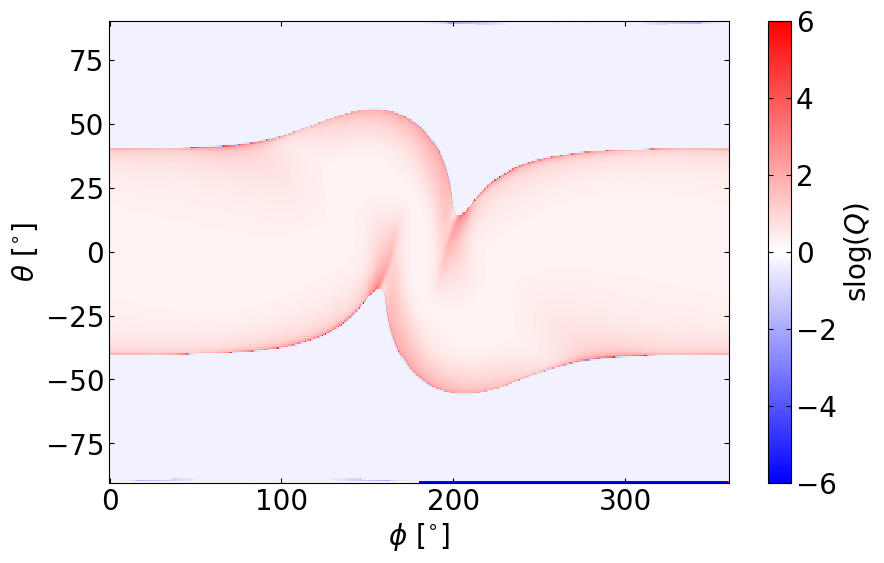
\includegraphics[scale=0.6]{Spherical_Example.png}
\end{center}

\newpage

(Optional) If you have the \texttt{Python} library \texttt{mayavi} installed, to can then execute the following command:

$\quad\quad$\texttt{./Run\_UFiT -g 1 -pp -nb -sf -b Example.bin -i Example2.inp -o Example2.flf}

This will use the same $B$-field as before, but calculate the fieldlines from a smaller set of start points; however, it will save the entire curve for each fieldline. Run the following script:

$\quad\quad$\texttt{python Visualize\_Spherical\_Example3D.py}

You should see the following 3D rendering in \texttt{mayavi} of $\mathrm{slog}(Q)$ on a surface and a selection of black fieldlines coming up from it.

\begin{center}
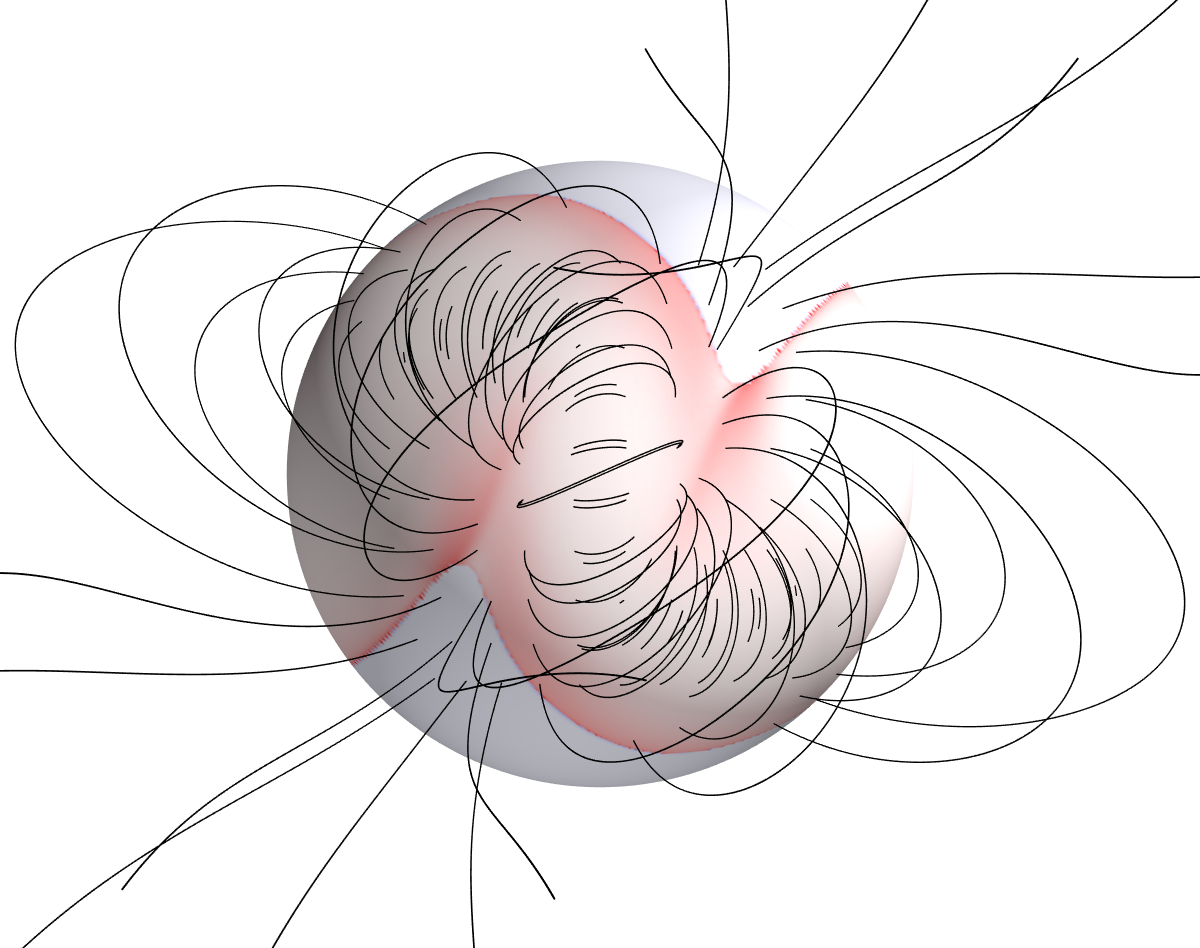
\includegraphics[scale=0.2]{Spherical_Example3D.png}
\end{center}

\vspace{2mm}
{\large \textbf{Example 2: (\texttt{Python} call) Synoptic Magnetogram}}

This example requires a few additional modules. Besides the usual, you will need to have the \texttt{Python} modules \texttt{wget}, \texttt{astropy}, \texttt{pfsspy} and \texttt{sunpy} installed. You can do this by setting up a virtual environment \textit{etc}, or executing the following (you may need to have administrator rights or add the suffix \texttt{-\,-user}):

$\quad\quad$\texttt{pip install astropy}

Open the script \texttt{HMI\_Example.py} for editing. Near the top, you should see the following line:

$\quad\quad$\texttt{UFiT\_home\_directory=\textquotesingle /change/this/path\textquotesingle }

This should be set to a path to where \texttt{UFiT} is installed. Now run the script by executing: 

$\quad\quad$\texttt{python HMI\_Example.py}

A synoptic magnetogram will be downloaded and a Potential Field Source Surface (PFSS) model be used to calculate $B$. This time, \texttt{Python} will call a compiled library directly, without the go-between of the input files and so on. You should see the following figure:

\begin{center}
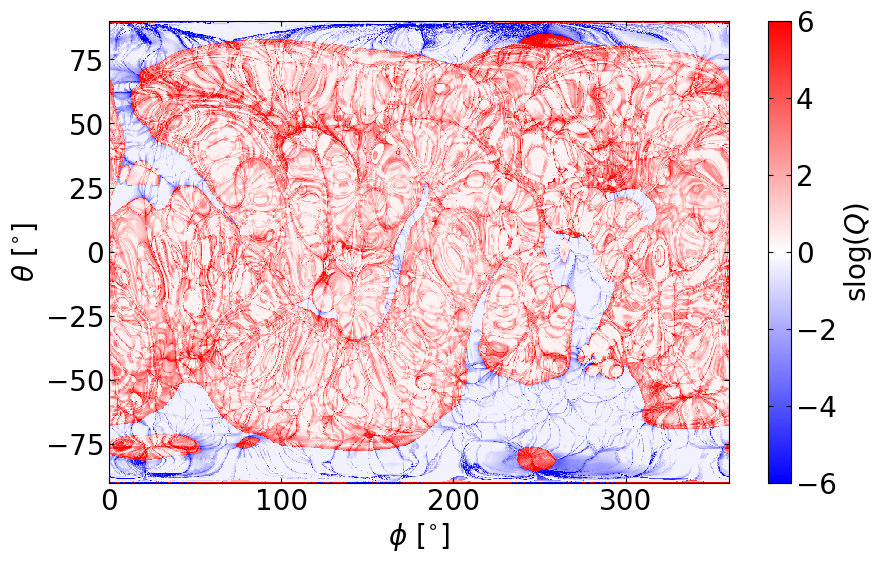
\includegraphics[scale=0.6]{HMI_Example.png}
\end{center}

The squashing factor is unsurprisingly busy, because the realistic data has not been filtered. Note that the original magnetogram has been downscaled for the purposes of the PFSS extrapolation and NaNs in the original data (in the poles where data is not available) replaced with zeros.


\vspace{2mm}
{\Large \textbf{Installation}}

Once the source code has been obtained, execute the following command to build the code:

$\quad\quad$\texttt{make}

This will follow the instructions in the \texttt{Makefile} to compile \texttt{UFiT}. If you wish to read \texttt{DUMFRIC} files directly, you will need to build \texttt{UFiT} with \texttt{netCDF} (instead, you can also use a \texttt{Python} script to convert them to a binary format first). Execute the following after substituting for the correct paths to the \texttt{netCDF} headers and library:

$\quad\quad$\texttt{make USE\_NC=True NC\_INCLUDE=/include/path NC\_LIB=/lib/path}

You can omit the arguments \texttt{NC\_INCLUDE} and \texttt{NC\_LIB} to use the defaults, or set them within the makefile directly.


\vspace{2mm}
{\Large \textbf{Running \texttt{UFiT} from the command line}}

Once this is done, you can run the executable as follows: 

$\quad\quad$\texttt{./Run\_UFiT}

You will need to add some command-line arguments from the tables below:

\vspace{2mm}

\begin{tabular}{|c|l|}		
		\hline
		\textbf{Argument} & \textbf{Effect} \\\hline\hline
		\texttt{-g} & \textbf{g}eometry: $0 =$ Cartesian; $1 =$ Spherical; $2 =$ Cylindrical  \\\hline
		\texttt{-r} & print available \textbf{r}esources (CPUs for now) \\\hline
		\texttt{-np} &  \textbf{n}umber of \textbf{p}rocessors (CPU) \\\hline
		\texttt{-cs} & \textbf{c}heck \textbf{s}tart points \\\hline
		\texttt{-px} & \textbf{p}eriodic \textbf{X} \\\hline
		\texttt{-py} & \textbf{p}eriodic \textbf{Y}  \\\hline
		\texttt{-pz} & \textbf{p}eriodic \textbf{Z}  \\\hline
		\texttt{-pp} & \textbf{p}eriodic $\phi$  \\\hline
		\texttt{-gs} & \textbf{g}rid \textbf{s}eparate or \textbf{s}taggered  \\\hline
		\texttt{-se} & \textbf{s}ave fieldline \textbf{e}ndpoints \\\hline
		\texttt{-sf} & \textbf{s}ave \textbf{f}ieldlines \\\hline
		\texttt{-sq} & \textbf{s}ave squashing factor $\mathbf{Q}$  \\\hline
		\texttt{-sc} & \textbf{s}ave \textbf{c}onnectivity type  \\\hline
		\texttt{-ud} & \textbf{u}ser \textbf{d}efined calculation  \\\hline
		\texttt{-nb} & normalized $B$ for $Q$ calculation; \textbf{this is highly recommended} \\\hline
		\texttt{-dl} & step size \\\hline
		\texttt{-ms} & \textbf{m}ax \textbf{s}teps  \\\hline
		\texttt{-i} & full path to \textbf{i}nput file (defining fieldline starts), \textit{e.g.} \texttt{./dir/ufit.inp} \\\hline
		\texttt{-c} & full path to \textbf{c}ommand file \textit{e.g.} \texttt{./dir/ufit.dat} \\\hline
		\texttt{-bt} & $\mathbf{B}$ file \textbf{t}ype (see below) \\\hline
		\texttt{-b} & full path to $\mathbf{B}$ file \textit{e.g.} \texttt{./dir/ufit.bin} \\\hline
		\texttt{-o} & full path to \textbf{o}utput file, \textit{e.g.} \texttt{./dir/out.flf} \\\hline

\end{tabular}

\vspace{2mm}

Add any combination of these arguments, as long as you include the correct option afterwards (\textit{e.g.} remembering to put \texttt{-o} followed by a space and then the path to the output file). The order of the arguements doesn't matter. For example, the command

$\quad\quad$\texttt{./Run\_UFiT -g 1 -pp -nb -sq -b B01.bin -o Q01.flf}

would calculate $Q$ in the spherical geometry (periodic longitude $\phi$), reading the magnetic field from \texttt{B01.bin} and writing the result to \texttt{Q01.flf}.


\vspace{2mm}
{\Large \textbf{(Optional) Running from a command file}}

When running from command line, the option \texttt{-c} can be used to specify a command file, from which the arguments can be read instead of through the command line. If no command line options are supplied, \texttt{UFiT} will automatically look for the default command file \texttt{ufit.dat} in the current working directory. The command file overwrites any command line arguments, if there is a conflict.

Each line in the command file specifies one argument, beginning with one of the following command codes, a semicolon and a space.

\begin{tabular}{|c|l|}		
		\hline
		\textbf{Code} & \textbf{Effect} \\\hline\hline
		\texttt{G:} & \textbf{g}eometry: $0 =$ Cartesian; $1 =$ Spherical; $2 =$ Cylindrical  \\\hline
		\texttt{R:} & print available \textbf{r}esources (CPUs for now) \\\hline
		\texttt{NP:} &  \textbf{n}umber of \textbf{p}rocessors (CPU) \\\hline
		\texttt{CS:} & \textbf{c}heck \textbf{s}tart points \\\hline
		\texttt{PX:} & \textbf{p}eriodic \textbf{X} \\\hline
		\texttt{PY:} & \textbf{p}eriodic \textbf{Y}  \\\hline
		\texttt{PZ:} & \textbf{p}eriodic \textbf{Z}  \\\hline
		\texttt{PP:} & \textbf{p}eriodic $\phi$  \\\hline
		\texttt{GS:} & \textbf{g}rid \textbf{s}eparate or \textbf{s}taggered  \\\hline
		\texttt{SE:} & \textbf{s}ave fieldline \textbf{e}ndpoints \\\hline
		\texttt{SF:} & \textbf{s}ave \textbf{f}ieldlines \\\hline
		\texttt{SQ:} & \textbf{s}ave squashing factor $\mathbf{Q}$  \\\hline
		\texttt{SC:} & \textbf{s}ave \textbf{c}onnectivity type  \\\hline
		\texttt{UD:} & \textbf{u}ser \textbf{d}efined calculation  \\\hline
		\texttt{NB:} & normalized $B$ for $Q$ calculation; \textbf{this is highly recommended} \\\hline
		\texttt{DL:} & step size \\\hline
		\texttt{MS:} & \textbf{m}ax \textbf{s}teps  \\\hline
		\texttt{I:} & full path to \textbf{i}nput file (defining fieldline starts), \textit{e.g.} \texttt{./dir/ufit.inp} \\\hline
		\texttt{BT:} & $\mathbf{B}$ file \textbf{t}ype (see below) \\\hline
		\texttt{B:} & full path to $\mathbf{B}$ file \textit{e.g.} \texttt{./dir/ufit.bin} \\\hline
		\texttt{O:} & full path to \textbf{o}utput file, \textit{e.g.} \texttt{./dir/out.flf} \\\hline

\end{tabular}


\vspace{2mm}
{\Large \textbf{Setting the fieldline start points}}

You will need to create an input file specifying the fieldline starts (sometimes called seeds). By default, it is called \texttt{ufit.inp} and contained in the current working directory; for any other name or location, specfity a valid path to it using the input file argument, \textit{e.g.} \texttt{-i ./somewhere/starts.something}

There are several input types which allow the fieldline starts to be specified in a convenient way.

\vspace{2mm}

\begin{tabular}{|c|l|}		
		\hline
		\textbf{Input type} & \textbf{Meaning} \\\hline\hline
		\texttt{0} & The coordinate of each start point is explicitly specified \\\hline
		\texttt{1} & Regular grid of start points where coordinates in each dimension  \\
		           & are explicitly defined  \\\hline
		\texttt{2} & Regular and equally spaced grid of start points in all dimensions; \\
		           & only a start and end point is specified for each dimension \\\hline
\end{tabular}

\vspace{2mm}

The first line of the input file must read 

$\quad\quad$\texttt{Input type: X}

where \texttt{X} must be one of the integers above. Thereafter, the structure depends on this type.

For \texttt{Input type:} \texttt{0} you must then put a single integer for the number of start points on the next line. On each subsequent line, you must put three comma-separated coordinates ($X,Y,Z$ or $r,\theta,\phi$ respectively). For example, in the following file three very different starts are specified:

\noindent\rule{\linewidth}{0.4pt}

$\quad\quad$\texttt{Input type: 0}

$\quad\quad$\texttt{3}

$\quad\quad$\texttt{0.3,0.0,0.1}

$\quad\quad$\texttt{0.7,0.2,0.3}

$\quad\quad$\texttt{0.5,-0.1,-5.0}

\noindent\rule{\linewidth}{0.4pt}

\vspace{2mm}

For \texttt{Input type:} \texttt{1} you must put three integers (each one on a new line) for the number of points in each dimension ($X,Y,Z$ or $r,\theta,\phi$ respectively). On each of the following lines, you must put comma-separated coordinates (as many as you have previously specified). For example, in the following file there are three points in $X$ (if Cartesian), four in $Y$ and one in $Z$; a total of twelve field lines will be traced.

\noindent\rule{\linewidth}{0.4pt}

$\quad\quad$\texttt{Input type: 1}

$\quad\quad$\texttt{3}

$\quad\quad$\texttt{4}

$\quad\quad$\texttt{1}

$\quad\quad$\texttt{-1.0,0.0,1.0}

$\quad\quad$\texttt{-0.5,0.5,1.5,2.5}

$\quad\quad$\texttt{10.0}

\noindent\rule{\linewidth}{0.4pt}

For \texttt{Input type:} \texttt{2} you must put three integers (each one on a new line) for the number of points in each dimension ($X,Y,Z$ or $r,\theta,\phi$ respectively). On each of the following lines, you must put comma-separated 

For example, in the following file there are 15 points in $X$ (if Cartesian), 10 in $Y$ and one in $Z$ for a total of 150 field lines. The fieldline starts will be spaced equally in $X$ from $-1$ to $1$ and so on.

\vspace{2mm}

\noindent\rule{\linewidth}{0.4pt}

$\quad\quad$\texttt{Input type: 2}

$\quad\quad$\texttt{15}

$\quad\quad$\texttt{10}

$\quad\quad$\texttt{1}

$\quad\quad$\texttt{-1.0,1.0}

$\quad\quad$\texttt{0.0,1.0}

$\quad\quad$\texttt{0.1,0.1}

\noindent\rule{\linewidth}{0.4pt}

\vspace{2mm}

In all cases, any more lines than are strictly necessary will be ignored. After making a valid input file as above, you may make several linebreaks and write some comments, store a previous configuration and so on. Only the first valid block will be used.

\vspace{2mm}
{\Large \textbf{Supported $B$ files}}

\texttt{UFiT} is intended to read the magnetic field from common MHD codes directly. By default, the type of file will be determined inherently from its extension (or start in the case of a \texttt{flicks}/\texttt{bfield} file from \texttt{ARMS}). Otherwise, you can use the command line argument \texttt{-bt} to specify which code created it, if you have changed the extension for example. The following table shows the currently supported file types and the code which goes after the argument \texttt{-bt} to manually specify them:

\vspace{2mm}
\begin{tabular}{|c|c|l|}		
		\hline
		\texttt{-bt} & \textbf{Default filename} & \textbf{Associated code} \\\hline\hline
		\texttt{-1} &  & Detect automatically \\\hline
		\texttt{0}  &  \texttt{.bin} & \texttt{UFiT} specific \\\hline
		\texttt{10} & \texttt{.nc} & \texttt{DUMFRIC} \\\hline
		\texttt{20} & \texttt{.sdf} & \texttt{Lare3d} \\\hline
		\texttt{30} & \texttt{flicks.} & \texttt{ARMS} \\\hline
		\texttt{31} & \texttt{bfield.} & \texttt{ARMS} \\\hline
\end{tabular}
\vspace{2mm}

If you have the magnetic field from some other source, you can always save it in the default \texttt{UFiT} format using the \texttt{Python} function \texttt{write\_B\_file()} (see below), or create a function in another language with the \texttt{Python} function as a reference.

{\large \textbf{Regular vs irregular grids}}

We define a ``regular'' 3-dimensional grid of points as one made up of 
 $\vec{v}_1 \otimes \vec{v}_2 \otimes \vec{v}_3$
In other words, this is the ordinary bunch of cuboids you think of when a 3-dimensional grid comes to mind. Note that the spacing between the points does not need to be constant, or identical, and nor does the number of points in each 
This is the preferred way to input the magnetic field to \texttt{UFiT}.

{\large \textbf{Separate (or staggered) grids}}

It is normally assumed that the $B$-field is defined on a single 3-dimensional grid, namely that at every grid point a vector $\vec{B}$ is completely known. A ``separate'' grid is one where each of the components of $B$ is defined at differing spatial locations. There are effectively three separate grids, which may have different numbers and separations of points. This means that, 
Each component of $B$ is then interpolated separately.


\vspace{2mm}
{\Large \textbf{Using \texttt{Python}}}

\vspace{2mm}
{\large \textbf{\texttt{Python} for plotting and analysis}}

\texttt{UFiT} is distributed along with a set of \texttt{Python} scripts. All the relevant functions and required libraries are contained in \texttt{UFiT\_Functions\_Python.py}. You will find example scripts for plotting and reading the \texttt{UFiT} outputs. Near the top of each of these is the following line

$\quad\quad$\texttt{UFiT\_home\_directory=\textquotesingle /change/this/path\textquotesingle }

which must be changed to instead contain a path to where the file \texttt{UFiT\_Functions\_Python.py} is kept. This way you can copy and modify the specific scripts for each task while keeping the main function library in one place (where you can also occasionally modify it).


\vspace{2mm}
{\large \textbf{(Optional) Calling routines directly from \texttt{Python}}}

You may create a \texttt{Python} script which calls compiled routines in \texttt{UFiT\_Python\_Callable.so} directly, without the go-between of calling from command line and writing in/outputs to disk. Example 2 above features just such a script.


\vspace{3mm}
{\Large \textbf{User defined calculations}}

You are, of course, free to change the source code as you see fit. The easiest way to run your own bespoke calculation might be to use the \texttt{user\_defined} or \texttt{-ud} option. You will then need to modify the file 

$\quad\quad$\texttt{UFiT\_User\_Functions.F90}

which by default contains three subroutines:
\begin{enumerate}
\item\texttt{prepare\_user\_defined} - called once initially, this gives you the opportunity to allocate memory, make preliminary calculations or read in additional files

\item\texttt{trace\_cartesian\_user} - main tracing routine which integrates forwards and back from a fieldline start if Cartesian coordinates are selected

\item\texttt{trace\_spherical\_user} - as above, for sphericals; feel free to leave this alone if you don't intend to use sphericals and vice versa
\end{enumerate}

The default version calculates $|\mathbf{B}|$ at each end of the field line and then saves the expansion factor $|\mathbf{B}_+|^2/|\mathbf{B}_-|^2$ as the user quantity. Any end quantity can be easily calculated by changing this directly. A quantity, such as a sum or a maximum, along field lines must be calculated by adding lines inside the two \texttt{do while} loops. Define and allocate additional variables as required.



\vspace{3mm}
{\Large \textbf{Visualization Routines}}


\end{document}
